\section{Numerical Illustration}
\label{sec:numerical_illustration}

This section presents the numerical illustration of the harmonic hosting capacity problem of a phase-balanced three-phase power system. To this end, first, a five bus section of a real-world industrial power system is considered to show the equivalence between the non-linear and second-order cone formulations. Second, a large-scale transmission system is considered, to show the scalability of the proposed second-order cone formulation. For the purpose of these numerical illustrations, any resistive impedance is scaled with a factor~$\sqrt{\Harmonic}$, and any inductive or capacitive impedance is appropriately scaled with a factor~$\Harmonic$. All results are presented in per-unit using a 100\,MVA basis.

\subsection{Industrial Power System}
\label{sec:industrial_power_system}

This numerical illustration considers a section of a real-world industrial phase-balanced three-phase power system across five voltage levels, with four transformers, three cables, and four harmonic units (Fig.~\ref{fig:industrial_network}). All necessary data for the harmonic hosting capacity problem can be derived from Fig.~\ref{fig:industrial_network}. On top of the fundamental harmonic, the considered harmonic set is $\HarmonicSet \in \{3,5,7\}$, i.e., one harmonic from each sequence subset. The aim of this numerical illustration is to 
\begin{enumerate*}
    \item validate the proposed formulations; and
    \item show the equivalence between the non-linear and second-order cone models.
\end{enumerate*}
For the purpose of proving equivalency, both models are solved using \textsc{Ipopt v1.6.2}~\cite{wachter_implementation_2006}, where the second-order constraints are translated to their equivalent non-convex quadratic form using the appropriate \textsc{MathOptInterface} constraint bridge~\cite{legat_mathoptinterface_2021}. 

\begin{figure*}
    \centering
    \begin{circuitikz}[scale = 0.68, transform shape]
        % Inf
        % 150 kV
        \draw (-2.00,0.00) node [above] {\large 0} to[short,*-] (-1.60,0.00) to[generic] (-0.40,0.00) -- (0.00,0.00);
        \draw (-2.00,1.00) to[short,*-] (-1.60,1.00) to[generic] (-0.40,1.00) -- (0.00,1.00);
        \draw (-2.00,2.00) to[short,*-] (-1.60,2.00) to[generic] (-0.40,2.00) -- (0.00,2.00);
        \draw (-2.00,0.00) edge[bend right,-latex] (-0.50,-1.50);
        \draw (-0.50,-1.50) node [right, align=left] {perfect inf. bus \\ $\ComplexVoltage_{0,1} = 1.0+j\,0.0$ \\ $\ComplexVoltage_{0,\Harmonic} = 0.0+j\,0.0$};
        % 150 kV
        \draw (0.00,0.00) node [above] {\large 1} to[short,*-] (0.50,0.00) to[L] (1.50,0.00) -- (2.00,0.00);
        \draw (0.00,1.00) to[short,*-] (0.50,1.00) to[L] (1.50,1.00) -- (2.00,1.00);
        \draw (0.00,2.00) to[short,*-] (0.50,2.00) to[L] (1.50,2.00) -- (2.00,2.00);
        \draw (2.00,2.00) -- (2.00,0.00); % to[normal open switch] (2.00,-3.00) node [eground] {};
        % 150-36kV
        \draw [dashed] (2.2,0.00) -- (2.2,5.50);
        % 36 kV
        \draw (2.50,0.00) to [L] (2.50,2.00) to[L] (4.23,1.00) to [L] (2.50,0.0);
        \draw (2.50,0.00) -- (4.50,0.00);
        \draw (4.23,1.00) -- (4.50,1.00);
        \draw (2.50,2.00) -- (4.50,2.00);
        \draw [fill=gray] (4.50,2.25) rectangle (4.75,-1.25);
        \draw (5.50,-2.0) node[isourceAMshape, fill=white, rotate=-90](I1){};
        \draw (I1.east) node [below,align=center] {$P_{\Unit_{1},1}$=50.00\,MW \\ $Q_{\Unit_{1},1}$=15.88\,Mvar \\ $\ComplexCurrent_{\Unit_{1},\Harmonic},~\forall \Harmonic \in \HarmonicSet\backslash\{1\}$};
        \draw (I1.west) -- (5.50,-0.5) -- (4.75,-0.5);
        % \draw   (3.75,-1.00) -- 
        %         ++({0.10*sin(30)},{-0.10*cos(30)}) 
        %             to [L, /tikz/circuitikz/bipoles/length=0.5cm] 
        %         ++({0.40*sin(30)},{-0.40*cos(30)}) -- 
        %         ++({0.10*sin(30)},{-0.10*cos(30)});
        % \draw   ({3.75+0.60*sin(30)},{-1.00-0.60*cos(30)}) -- 
        %         ++({-0.10*sin(30)},{-0.10*cos(30)}) 
        %             to [L, /tikz/circuitikz/bipoles/length=0.5cm] 
        %         ++({-0.40*sin(30)},{-0.40*cos(30)}) -- 
        %         ++({-0.10*sin(30)},{-0.10*cos(30)});
        % \draw   (3.75,-2.06) -- 
        %         ++({-0.10*sin(90)},{-0.10*cos(90)}) 
        %             to [L, /tikz/circuitikz/bipoles/length=0.5cm] 
        %         ++({-0.40*sin(90)},{-0.40*cos(90)}) -- 
        %         ++({-0.10*sin(90)},{-0.10*cos(90)});
        % \draw   ({3.75-0.60*sin(90)},{-2.06-0.60*cos(90)}) -- 
        %         ++({-0.10*sin(45)},{-0.10*cos(45)}) 
        %             to [L, /tikz/circuitikz/bipoles/length=0.5cm] 
        %         ++({-0.40*sin(45)},{-0.40*cos(45)}) -- 
        %         ++({-0.10*sin(45)},{-0.10*cos(45)});
        % \draw   (3.75,-2.06) -- 
        %         ++({0.10*sin(45)},{-0.10*cos(45)}) 
        %             to [L, /tikz/circuitikz/bipoles/length=0.5cm] 
        %         ++({0.40*sin(45)},{-0.40*cos(45)}) -- 
        %         ++({0.10*sin(45)},{-0.10*cos(45)});
        % \draw   ({3.75+0.60*sin(45)},{-2.06-0.60*cos(45)}) -- 
        %         ++({0.10*sin(90)},{-0.10*cos(90)}) 
        %             to [L, /tikz/circuitikz/bipoles/length=0.5cm] 
        %         ++({0.40*sin(90)},{-0.40*cos(90)}) -- 
        %         ++({0.10*sin(90)},{-0.10*cos(90)});
        % \draw   (3.75,-2.06) -- (3.75,-3.00) node [eground] {};
        % \draw   ({3.75+0.60*(sin(45)+sin(90)},2.00) --
        %         ({3.75+0.60*(sin(45)+sin(90)},{-2.06-0.60*(cos(45)+cos(90)});
        % \draw   ({3.75+0.60*(sin(45)+sin(90)-0.25},1.00) -- 
        %         ({3.75+0.60*(sin(45)+sin(90)-0.25},-0.66) --
        %         (3.75,-0.66) -- (3.75,-1.00);
        % \draw   ({3.75+0.60*(sin(45)+sin(90)-0.50},1.00) --
        %         ({3.75+0.60*(sin(45)+sin(90)-0.50},-0.33) --
        %         ({3.75-0.60*(sin(90)+sin(45))},-0.33) -- 
        %         ({3.75-0.60*(sin(90)+sin(45))},{-2.06-0.60*(cos(90)+sin(45))});
        \draw   (4.75,0.00) -- (5.00,0.00) node [above] {\large 2} to [short,*-*] (6.00,0.00) node [above] {\large 3} -- (6.50,0.00) to[L] (8.00,0.00) -- (8.50,0.00);
        \draw   (4.75,1.00) -- (5.00,1.00) to [short,*-*] (6.00,1.00) -- (6.50,1.00) to[L] (8.00,1.00) -- (8.50,1.00);
        \draw   (4.75,2.00) -- (5.00,2.00) to [short,*-*] (6.00,2.00) -- (6.50,2.00) to[L] (8.00,2.00) -- (8.50,2.00);
        \draw   (8.50,2.00) -- (8.50,-0.00); % to [gf surge arrester] (8.50,-3.00) node [eground] {};
        % 36 - 10 kV
        \draw   [dashed] (8.75,0.00) -- (8.75,5.50);
        % 10 kV
        \draw (9.00,0.00) -- (9.50,0.00) to[L] (10.50,0.00) -- (11.00,0.00);
        \draw (9.00,1.00) -- (9.50,1.00) to[L] (10.50,1.00) -- (11.00,1.00);
        \draw (9.00,2.00) -- (9.50,2.00) to[L] (10.50,2.00) -- (11.00,2.00);
        \draw (9.00,2.00) -- (9.00,-0.00); % to [gf surge arrester] (9.00,-3.00) node [eground] {};
        \draw [fill=gray] (11.00,2.25) rectangle (11.25,-1.25);
        \draw (12.00,-2.0) node[isourceAMshape, fill=white, rotate=-90](I2){};
        \draw (I2.east) node [below,align=center] {$P_{\Unit_{2},1}$=12.60\,MW \\ $Q_{\Unit_{2},1}$=4.00\,Mvar \\ $\ComplexCurrent_{\Unit_{2},\Harmonic},~\forall \Harmonic \in \HarmonicSet\backslash\{1\}$};
        \draw (I2.west) -- (12.00,-0.5) -- (11.25,-0.5);
        % \draw   (11.75,-3.50) to [C, /tikz/circuitikz/bipoles/length=0.5cm] (11.75,-2.20);
        % \draw   (12.50,-3.50) to [C, /tikz/circuitikz/bipoles/length=0.5cm] (12.50,-2.20);
        % \draw   (13.25,-3.50) to [C, /tikz/circuitikz/bipoles/length=0.5cm] (13.25,-2.20);
        % \draw   (11.75,-3.50) -- (13.25,-3.50);
        % \draw   (11.75,-2.20) -- (11.75,-2.00) to [L] (11.75,-1.00) -- (11.75,-0.90) -- (11.25,-0.90);
        % \draw   (12.50,-2.20) -- (12.50,-2.00) to [L] (12.50,-1.00) -- (12.50,-0.60) -- (11.25,-0.60);
        % \draw   (13.25,-2.20) -- (13.25,-2.00) to [L] (13.25,-1.00) -- (13.25,-0.30) -- (11.25,-0.30);
        \draw   (11.25,0.00) -- (11.50,0.00) node [above] {\large 4} to [short,*-*] (12.50,0.00) node [above] {\large 5} -- (14.73,0.00);
        \draw   (11.25,1.00) -- (11.50,1.00) to [short,*-*] (12.50,1.00) -- (13.00,1.00);
        \draw   (11.25,2.00) -- (11.50,2.00) to [short,*-*] (12.50,2.00) -- (14.73,2.00);
        \draw   (14.73,0.00) to [L] (14.73,2.00) to[L] (13.00,1.00) to [L] (14.73,0.0);
        % 10 kV - 690 V
        \draw   [dashed] (14.95,0.00) -- (14.95,5.50);
        % 690 V
        \draw (15.25,-1.00) -- (17.25,-1.00);
        \draw (15.25,0.00) -- (15.75,0.00) to[L] (16.75,0.00) -- (17.25,0.00);
        \draw (15.25,1.00) -- (15.75,1.00) to[L] (16.75,1.00) -- (17.25,1.00);
        \draw (15.25,2.00) -- (15.75,2.00) to[L] (16.75,2.00) -- (17.25,2.00);
        \draw (15.25,2.00) -- (15.25,0.00) to [short] (15.25,-2.50) node [eground] {};
        \draw (15.25,-1.00) node [below right,align=left] {\footnotesize PEN (Al) \\ \footnotesize 500\,mm$^{\text{2}}$ \\ \footnotesize 15\,m};
        \draw [fill=gray] (17.25,2.25) rectangle (17.50,-1.25);
        \draw (18.25,-2.0) node[isourceAMshape, fill=white, rotate=-90](I3){};
        \draw (I3.east) node [below,align=center] {$P_{\Unit_{3},1}$=1.42\,MW \\ $Q_{\Unit_{3},1}$=0.00\,Mvar \\ $\ComplexCurrent_{\Unit_{3},\Harmonic},~\forall \Harmonic \in \HarmonicSet\backslash\{1\}$};
        \draw (I3.west) -- (18.25,-0.5) -- (17.5,-0.5);
        % \draw   (18.00,-3.50) to [C, /tikz/circuitikz/bipoles/length=0.5cm]
        %         (19.50,-3.50) to[C, /tikz/circuitikz/bipoles/length=0.5cm]
        %         (18.75,-2.20) to [C, /tikz/circuitikz/bipoles/length=0.5cm] (18.00,-3.50);
        % \draw   (18.00,-3.50) -- (18.00,-2.00) to [L] (18.00,-1.00) -- (18.00,-0.90) -- (17.50,-0.90);
        % \draw   (18.75,-2.20) -- (18.75,-2.00) to [L] (18.75,-1.00) -- (18.75,-0.60) -- (17.50,-0.60);
        % \draw   (19.50,-3.50) -- (19.50,-2.00) to [L] (19.50,-1.00) -- (19.50,-0.30) -- (17.50,-0.30);
        \draw   (17.50,0.00) -- (17.75,0.00) node [above] {\large 6} to [short,*-*] (18.75,0.00) node [above] {\large 7} -- (20.98,0.00);
        \draw   (17.50,1.00) -- (17.75,1.00) to [short,*-*] (18.75,1.00) -- (19.25,1.00);
        \draw   (17.50,2.00) -- (17.75,2.00) to [short,*-*] (18.75,2.00) -- (20.98,2.00);
        \draw (20.98,0.00) to [L] (20.98,2.00) to[L] (19.25,1.00) to [L] (20.98,0.0);
        % 690 V - 400 V
        \draw   [dashed] (21.30,0.00) -- (21.30,5.50);
        % 400 V
        \draw   (22.50,2.00) -- 
                ++({0.10*sin(30)},{-0.10*cos(30)}) 
                    to [L, /tikz/circuitikz/bipoles/length=0.5cm] 
                ++({0.40*sin(30)},{-0.40*cos(30)}) -- 
                ++({0.10*sin(30)},{-0.10*cos(30)});
        \draw   ({22.50+0.60*sin(30)},{2.00-0.60*cos(30)}) -- 
                ++({-0.10*sin(30)},{-0.10*cos(30)}) 
                    to [L, /tikz/circuitikz/bipoles/length=0.5cm] 
                ++({-0.40*sin(30)},{-0.40*cos(30)}) -- 
                ++({-0.10*sin(30)},{-0.10*cos(30)});
        \draw   (22.50,0.96) -- 
                ++({-0.10*sin(90)},{-0.10*cos(90)}) 
                    to [L, /tikz/circuitikz/bipoles/length=0.5cm] 
                ++({-0.40*sin(90)},{-0.40*cos(90)}) -- 
                ++({-0.10*sin(90)},{-0.10*cos(90)});
        \draw   ({22.50-0.60*sin(90)},{0.96-0.60*cos(90)}) -- 
                ++({-0.10*sin(45)},{-0.10*cos(45)}) 
                to [L, /tikz/circuitikz/bipoles/length=0.5cm] 
                ++({-0.40*sin(45)},{-0.40*cos(45)}) -- 
                ++({-0.10*sin(45)},{-0.10*cos(45)});
        \draw   (22.50,0.96) -- 
                ++({0.10*sin(45)},{-0.10*cos(45)}) 
                    to [L, /tikz/circuitikz/bipoles/length=0.5cm] 
                ++({0.40*sin(45)},{-0.40*cos(45)}) -- 
                ++({0.10*sin(45)},{-0.10*cos(45)});
        \draw   ({22.50+0.60*sin(45)},{0.96-0.60*cos(45)}) -- 
                ++({0.10*sin(90)},{-0.10*cos(90)}) 
                    to [L, /tikz/circuitikz/bipoles/length=0.5cm] 
                ++({0.40*sin(90)},{-0.40*cos(90)}) -- 
                ++({0.10*sin(90)},{-0.10*cos(90)});
        \draw   (22.50,2.00) to [short,-*] (23.75,2.00) -- (24.00,2.00);
        \draw   (22.50,0.96) -- (22.50,0.00) to [short] (22.50,-2.50) node [eground] {};
        \draw   (22.50,-1.00) node [below right,align=left] {\footnotesize PEN (Cu) \\ \footnotesize 120\,mm$^{\text{2}}$ \\ \footnotesize 30\,m};
        \draw   (22.50,-1.00) -- (24.00,-1.00);
        \draw   ({22.50+0.60*(sin(45)+sin(90)},{0.96-0.60*(cos(45)+cos(90))}) to [short,-*] (23.75,{0.96-0.60*(cos(45)+cos(90))}) --
                (24.00,{0.96-0.60*(cos(45)+cos(90))});
        \draw   ({22.50-0.60*(sin(90)+sin(45))},{0.96-0.60*(cos(90)+sin(45))}) --
                ({22.50-0.60*(sin(90)+sin(45))},0.00) to [short,-*] (23.75,0.00) node [above] {\large 8} -- 
                (24.00,0.00);
        \draw   [fill=gray] (24.00,2.25) rectangle (24.25,-1.25);
        \draw (24.125,-2.0) node[isourceAMshape, fill=white, rotate=-90](I4){};
        \draw (I4.east) node [below,align=center] {$P_{\Unit_{4},1}$=0.05\,MW \\ $Q_{\Unit_{4},1}$=0.04\,Mvar \\ $\ComplexCurrent_{\Unit_{4},\Harmonic},~\forall \Harmonic \in \HarmonicSet\backslash\{1\}$};
        \draw (I4.west) -- (24.125,-1.25);
        % labels
        \draw [dashed] (-2.00,4.05) -- (24.25,4.05);
        \draw (0.00,4.70) [align=center] node {\large 155.0\,kV \\ 0.94$\leq\Voltage^{\text{rms}}\leq$1.06 \\ IEC61000-3-6:2008};
        \draw (5.500,4.70) [align=center] node {\large 35.4\,kV \\ 0.94$\leq\Voltage^{\text{rms}}\leq$1.06 \\ IEC61000-2-4:2002};
        \draw (11.825,4.70) [align=center] node {\large 10.0\,kV \\ 0.90$\leq\Voltage^{\text{rms}}\leq$1.10 \\ IEC61000-2-4:2002};
        \draw (18.125,4.70) [align=center] node {\large 690.0\,V \\ 0.90$\leq\Voltage^{\text{rms}}\leq$1.10 \\ IEC61000-2-4:2002};
        \draw (22.750,4.70) [align=center] node {\large 400.0\,V \\ 0.90$\leq\Voltage^{\text{rms}}\leq$1.10 \\ IEC61000-2-4:2002};
        \draw (-1.00,3.20) node [align=center] {S$^{\text{sc}}$=2.1\,GVA \\ XRr=20};
        \draw (2.15,3.20) node [fill=white, align=center] { 150/36\,kV\,$\|$\,125\,MVA \\ 
                                                            ~~~\,\,\,u$_{k}$=17\,\%\,$\|$\,P$_{k}$=527\,kW \\ 
                                                            P$_{0}$=77.5\,kW$\|$Yd11~~~~~~\,\,}; 
        \draw (8.575,3.20) node [fill=white, align=center] {~~~36/10\,kV\,$\|$\,31.5\,MVA \\ 
                                                            ~~\,u$_{k}$=12.5\,\%\,$\|$\,P$_{k}$=99\,kW \\
                                                            P$_{0}$=14.2\,kW\,$\|$\,Yy0~~~~~~\, }; 
        \draw (14.8,3.20) node [fill=white, align=center] {~10/0.69\,kV\,$\|$\,3.15\,MVA \\ 
                                                            ~~~~\,\,\,u$_{k}$=6\,\%\,$\|$\,P$_{k}$=20\,kW \\
                                                            P$_{0}$=2.7\,kW\,$\|$\,Dyn11~~~~};
        \draw (21.225,3.20) node [fill=white, align=center] {690/400\,V\,$\|$\,250\,kVA \\ 
                                                            ~~~\,\,u$_{k}$=2.5\,\%\,$\|$\,P$_{k}$=1.6\,kW \\
                                                            P$_{0}$=1.0\,kW\,$\|$\,Dzn0~~~~\,};
        \draw (5.50,3.25) node [align=center] {NA2XS(FL)2Y \\ 3x1x400/35\,mm$^{2}$ \\ 1500\,m};
        \draw (12.00,3.25) node [align=center] {NA2XS(F)2Y \\ 3x1x240/25\,mm$^{2}$ \\ 200\,m};
        \draw (18.25,3.25) node [align=center] {NYY \\ 3x240/120\,mm$^{2}$ \\ 70\,m};
        % \draw (19.50,-2.85) node [right] {400\,kvar};
        % \draw (13.50,-2.85) node [right] {6\,Mvar};
    \end{circuitikz}
    \caption{Section of a real-world industrial phase-balanced three-phase power system across five voltage levels with their root-mean-square voltage limits and applicable harmonic voltage standard, with four transformers, three cables, and four harmonic units with their fundamental power consumption.}
    \label{fig:industrial_network}
\end{figure*}

\begin{figure}
    \centering
    \subfloat[zero seq. (h=3), axes are rotated by -90$^{\circ}$ \label{fig:zero_seq_results}]
    {
    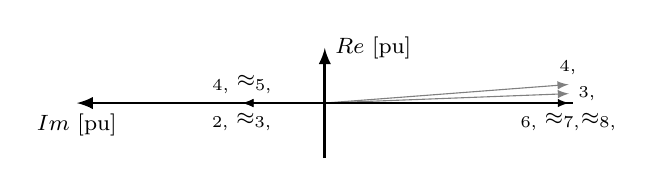
\begin{tikzpicture}[scale=70,rotate=90]
        % axis
        \draw[line width=1.0pt,-latex] (-0.010,0.0)--(0.010,0.0) node[right] {\footnotesize $\mathfrak{Re}$ [pu]};
        \draw[line width=1.0pt,-latex] (0.0,-0.045)--(0.0,0.045) node[below] {\footnotesize $\mathfrak{Im}$ [pu]};
        % coordinates - bus voltage
        \coordinate (orig)  at ( 0.00000, 0.00000);
        \coordinate (U0)    at (0.0,-0.0);
        \coordinate (U1)    at (0.0,0.0);
        \coordinate (U2)    at (-0.0,0.0154);
        \coordinate (U3)    at (0.0,0.01541);
        \coordinate (U4)    at (-0.0,0.01534);
        \coordinate (U5)    at (0.0,0.01534);
        \coordinate (U6)    at (-1.0e-5,-0.04556);
        \coordinate (U7)    at (-1.0e-5,-0.04556);
        \coordinate (U8)    at (-1.0e-5,-0.0455);
        \coordinate (E1)    at (0.0,-0.0);
        \coordinate (E2)    at (0.0,0.0);
        \coordinate (E3)    at (0.00176,-0.04556);
        \coordinate (E4)    at (0.00347,-0.0455);
        % vectors - xfmr excitation 
        % \draw[-latex, gray] (orig) -- (E1) node[black, anchor=west]{\footnotesize $\ComplexExcitationVoltage_{1,\Harmonic}$};
        % \draw[-latex, gray] (orig) -- (E2) node[black, anchor=east]{\footnotesize $\ComplexExcitationVoltage_{2,\Harmonic}$};
        \draw[-latex, gray] (orig) -- (E3) node[black, anchor=west]{\footnotesize $\ComplexExcitationVoltage_{3,\Harmonic}$};
        \draw[-latex, gray] (orig) -- (E4) node[black, anchor=south]{\footnotesize $\ComplexExcitationVoltage_{4,\Harmonic}$};
        % vectors - bus voltage
        % \draw[-latex] (orig) -- (U1) node[anchor=north]{\footnotesize $\ComplexVoltage_{1,\Harmonic}$};
        \draw[-latex] (orig) -- (U2) node[anchor=north]{\footnotesize $\ComplexVoltage_{2,\Harmonic} \approx \ComplexVoltage_{3,\Harmonic}$};
        \draw[-latex] (orig) -- (U4) node[anchor=south]{\footnotesize $\ComplexVoltage_{4,\Harmonic} \approx \ComplexVoltage_{5,\Harmonic}$};
        \draw[-latex] (orig) -- (U6) node[anchor=north]{\footnotesize $\ComplexVoltage_{6,\Harmonic} \approx \ComplexVoltage_{7,\Harmonic}\approx\ComplexVoltage_{8,\Harmonic}$};
    \end{tikzpicture}
    }
    \hfill 
    \subfloat[neg. seq. (h=5) \label{fig:neg_seq_results}]
    {
    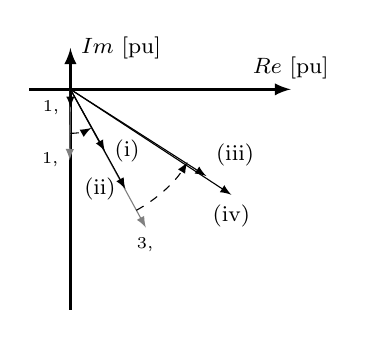
\begin{tikzpicture}[scale=70]
        % axis
        \draw[line width=1.0pt,-latex] (-0.0075,0.0)--(0.040,0.0) node[above] {\footnotesize $\mathfrak{Re}$ [pu]};
        \draw[line width=1.0pt,-latex] (0.0,-0.040)--(0.0,0.0075) node[right] {\footnotesize $\mathfrak{Im}$ [pu]};
        % coordinates - bus voltage
        \coordinate (orig)  at ( 0.00000, 0.00000);
        \coordinate (U0)    at (-0.0,0.0);
        \coordinate (U1)    at (-8.0e-5,-0.00332);
        \coordinate (U2)    at (0.00625,-0.01121);
        \coordinate (U3)    at (0.00628,-0.01149);
        \coordinate (U4)    at (0.00998,-0.01808);
        \coordinate (U5)    at (0.00997,-0.01817);
        \coordinate (U6)    at (0.02427,-0.01509);
        \coordinate (U7)    at (0.02466,-0.01573);
        \coordinate (U8)    at (0.0292,-0.01914);
        \coordinate (E1)    at (-0.00014,-0.01283);
        \coordinate (E2)    at (0.01002,-0.01806);
        \coordinate (E3)    at (0.01368,-0.02508);
        \coordinate (E4)    at (0.02937,-0.01885);
        % vectors - xfmr excitation 
        \draw[-latex, gray] (orig) -- (E1) node[black, anchor=east]{\footnotesize $\ComplexExcitationVoltage_{1,\Harmonic}$};
        %\draw[-latex, gray] (orig) -- (E2) node[black, anchor=east]{\footnotesize $\ComplexExcitationVoltage_{2,\Harmonic}$};
        \draw[-latex, gray] (orig) -- (E3) node[black, anchor=north]{\footnotesize $\ComplexExcitationVoltage_{3,\Harmonic}$};
        % \draw[-latex, gray] (orig) -- (E4) node[black, anchor=north]{\footnotesize $\ComplexExcitationVoltage_{4,\Harmonic}$};
        % vectors - bus voltage
        \draw[-latex] (orig) -- (U1) node[anchor=east]{\footnotesize $\ComplexVoltage_{1,\Harmonic}$};
        \draw[-latex] (orig) -- (U2) node[anchor=west]{\footnotesize (i)}; %~~~\ComplexVoltage_{2,\Harmonic} \approx \ComplexVoltage_{3,\Harmonic}
        \draw[-latex] (orig) -- (U4) node[anchor=east]{\footnotesize (ii)}; %$\ComplexExcitationVoltage_{2,\Harmonic} \approx \ComplexVoltage_{4,\Harmonic} \approx \ComplexVoltage_{5,\Harmonic}$
        % \draw[-latex] (orig) -- (U6) node[anchor=west]{\footnotesize $\ComplexVoltage_{6,\Harmonic}$};
        \draw[-latex] (orig) -- (U7) node[anchor=south west]{\footnotesize (iii)}; %$\ComplexVoltage_{6,\Harmonic}\approx\ComplexVoltage_{7,\Harmonic}$
        \draw[-latex] (orig) -- (U8) node[anchor=north]{\footnotesize (iv)};%$\ComplexExcitationVoltage_{4,\Harmonic}\approx\ComplexVoltage_{8,\Harmonic}$};
        % angle shift - xfmr 
        \draw [-latex, dashed] (8.841583e-5,-0.007999) arc [radius=0.008, start angle=-89.36675, end angle=-60.8686715]; 
        \draw [-latex, dashed] (0.011968,-0.02194879) arc [radius=0.025, start angle=-61.396275, end angle=-31.869292];
    \end{tikzpicture}
    }
    % \hfill 
    \subfloat[pos. seq. (h=7) \label{fig:pos_seq_results}]
    {
    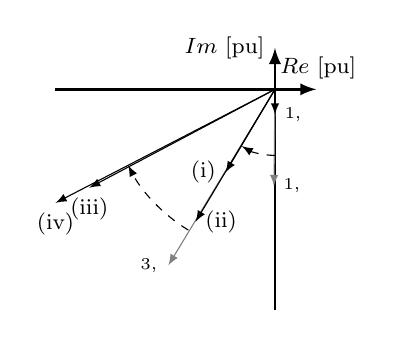
\begin{tikzpicture}[scale=70]
        % axis
        \draw[line width=1.0pt,-latex] (-0.040,0.00)--(0.0075,0.00) node[above] {\footnotesize $\,\mathfrak{Re}$ [pu]};
        \draw[line width=1.0pt,-latex] (0.0,-0.040)--(0.00,0.0075) node[left] {\footnotesize $\mathfrak{Im}$ [pu]};
        % coordinates - bus voltage
        \coordinate (orig)  at ( 0.00000, 0.00000);
        \coordinate (U0)    at (0.0,0.0);
        \coordinate (U1)    at (-9.0e-5,-0.00454);
        \coordinate (U2)    at (-0.00897,-0.01507);
        \coordinate (U3)    at (-0.00926,-0.01531);
        \coordinate (U4)    at (-0.01441,-0.02402);
        \coordinate (U5)    at (-0.0145,-0.02406);
        \coordinate (U6)    at (-0.03284,-0.01779);
        \coordinate (U7)    at (-0.0337,-0.01786);
        \coordinate (U8)    at (-0.03983,-0.0206);
        \coordinate (E1)    at (-0.00018,-0.01753);
        \coordinate (E2)    at (-0.01437,-0.02404);
        \coordinate (E3)    at (-0.01935,-0.03194);
        \coordinate (E4)    at (-0.03966,-0.02089);
        % vectors - xfmr excitation 
        \draw[-latex, gray] (orig) -- (E1) node[black, anchor=west]{\footnotesize $\ComplexExcitationVoltage_{1,\Harmonic}$};
        % \draw[-latex, gray] (orig) -- (E2) node[black, anchor=east]{\footnotesize $\ComplexExcitationVoltage_{2,\Harmonic}$};
        \draw[-latex, gray] (orig) -- (E3) node[black, anchor=east]{\footnotesize $\ComplexExcitationVoltage_{3,\Harmonic}$};
        % \draw[-latex, gray] (orig) -- (E4) node[black, anchor=east]{\footnotesize $\ComplexExcitationVoltage_{4,\Harmonic}$};
        % vectors - bus voltage
        \draw[-latex] (orig) -- (U1) node[anchor=west]{\footnotesize $\ComplexVoltage_{1,\Harmonic}$};
        \draw[-latex] (orig) -- (U2) node[anchor=east]{\footnotesize (i)}; %$\ComplexVoltage_{2,\Harmonic} \approx \ComplexVoltage_{3,\Harmonic}$
        \draw[-latex] (orig) -- (U4) node[anchor=west]{\footnotesize (ii)};
        % \draw[-latex] (orig) -- (U6) node[anchor=north]{\footnotesize $\ComplexVoltage_{6,\Harmonic}$};
        \draw[-latex] (orig) -- (U7) node[anchor=north]{\footnotesize (iii)};
        \draw[-latex] (orig) -- (U8) node[anchor=north]{\footnotesize (iv)};
        % angle shift - xfmr 
        \draw [-latex, dashed] (0.00000000,-0.012000) arc [radius=0.012, start angle=269.3793, end angle=239.1803]; 
        \draw [-latex, dashed] (-0.0157241,-0.025549) arc [radius=0.030, start angle=238.3897, end angle=207.3686];
    \end{tikzpicture}
    }
    \caption{The bus and excitation voltage phasors throughout the industrial power system (Fig.~\ref{fig:industrial_network}) for (a) zero, (b) negative, and (c) positive sequence, respectively, for the non-linear model with the Kalai-Smorodinsky bargaining fairness objective, where (i) $\ComplexVoltage_{2,\Harmonic} \approx \ComplexVoltage_{3,\Harmonic}$, (ii) $\ComplexExcitationVoltage_{2,\Harmonic} \approx \ComplexVoltage_{4,\Harmonic} \approx \ComplexVoltage_{5,\Harmonic}$, (iii) 
    $\ComplexVoltage_{6,\Harmonic}\approx\ComplexVoltage_{7,\Harmonic}$, and (iv) $\ComplexExcitationVoltage_{4,\Harmonic}\approx\ComplexVoltage_{8,\Harmonic}$.}
    \label{fig:voltage_results}
\end{figure}

\subsubsection{Validate the proposed formulation} 

It should be noted that the purpose of this numerical illustration is not to provide realistic results for an industrial power system, rather validate correct implementation of the presented mathematical framework. Consequently, for the purpose of validating the proposed formulation, the non-linear model is considered with the Kalai-Smorodinsky bargaining fairness objective. The Kalai-Smorodinsky bargaining fairness objective ensures that 
\begin{enumerate*}
    \item [(i)] individual harmonic voltage distortion at all busses approach their limits, resulting in harmonic voltages of similar magnitudes at every bus; and
    \item [(ii)] all units inject at least a minimum amount of harmonic current (Table~\ref{tab:unit_currents}), 
\end{enumerate*}
allowing easier validation. 

\begin{table}[b!]
    \centering
    \caption{Harmonic current injection for the non-linear model with the Kalai-Smorodinsky bargaining fairness objective.}
    \label{tab:unit_currents}
    \begin{tabular}{c | c c c c c c}
        \multirow{2}{*}{unit}   & \multicolumn{2}{c}{h=3}                                           & \multicolumn{2}{c}{h=5}                       & \multicolumn{2}{c}{h=7}                       \\ 
                                & $|\ComplexCurrent|$\,[pu] & $\angle\ComplexCurrent$\,[$^{\circ}$] & $|\ComplexCurrent|$\,[pu] & $\angle\ComplexCurrent$\,[$^{\circ}$] & $|\ComplexCurrent|$\,[pu] & $\angle\ComplexCurrent$\,[$^{\circ}$] \\ \hline
        $\Unit_{1}$             & 0.0000740                & 0.0                        & 0.0100655                      & 30.0                 & 0.0098060       & -30.0                      \\
        $\Unit_{2}$             & 0.0000013                & 0.0                        & 0.0031490                      & 30.0                 & 0.0030833       & -30.0                      \\
        $\Unit_{3}$             & 0.0063852                & 0.0                        & 0.0005429                      & 60.0                 & 0.0004568       & -60.0                      \\
        $\Unit_{4}$             & 0.0015689                & 0.0                        & 0.0001167                      & 60.0                 & 0.0000987       & -60.0                      \\
    \end{tabular}
\end{table}

Fig.~\ref{fig:voltage_results} shows the voltage phasors throughout the industrial power system for the
\begin{enumerate*}
    \item [(a)] zero ($3^{rd}$ harmonic),
    \item [(b)] negative ($5^{th}$ harmonic), and
    \item [(c)] positive sequence $37{th}$ harmonic, respectively.
\end{enumerate*}
Fig.~\ref{fig:zero_seq_results} shows that, for the zero-sequence harmonics, the transformers successfully decouple the different voltage levels of the system. Fig.~\ref{fig:neg_seq_results} and~\ref{fig:pos_seq_results} show that the fifth and seventh harmonic voltage~$\ComplexVoltage_{1,h}$ at bus one is approximately 25.9\,\% of the excitation voltage~$\ComplexExcitationVoltage_{1,h}$ at transformer one, which is inline with the ratio between the short-circuit impedance of the infinite grid and the first transformer. Using a dashed arc, Fig.~\ref{fig:neg_seq_results} and~\ref{fig:pos_seq_results} show the phase-shift of approximately thirty degrees, respectively counter-clockwise and clockwise, between the excitation and secondary voltage of the first and fourth transformer. Furthermore, a phase-shift of approximately zero degrees between the excitation and secondary voltage of the second and third transformer. Note that the phase-shift is not exactly zero or thirty degrees as it also includes the voltage drop over the secondary winding resistance.

\subsubsection{Equivalence between the non-linear and second-order cone model} 

\begin{table}[b!]
    \centering
    \caption{Objective value and solve times of non-linear and second- order cone models, for each considered fairness objective.}
    \label{tab:equivalence}
    \begin{tabular}{l l | c c c c c c}
    obj.                        & mod.      & obj. value                    & \multicolumn{4}{c}{solve time [s]\footnote{The solve times are split in the individual components for the preceding calculation to determine maximum harmonic current injection of each harmonic unit (pre.), fundamental power flow (fpf), and harmonic hosting capacity (hhc), when applicable. Lastly, the total solve time (tot.) is given.}}    \\ \cline{4-7}
                                &           &                               & pre.  & fpf   & hhc   & tot.          \\ \hline
    \multirow{2}{*}{abs. eq.}   & nl        & 0.00395625133\underline{9}    & -     & -     & 0.53  & 0.53          \\
                                & soc       & 0.00395625133\underline{8}    & -     & 0.06  & 0.17  & 0.23          \\ \arrayrulecolor{gray!20} \hline
    \multirow{2}{*}{max. eff.}  & nl        & 0.0970450321\underline{96}    & -     & -     & 0.82 & 0.82         \\
                                & soc       & 0.0970450321\underline{88}    & -     & 0.07 & 0.35 & 0.42         \\ \arrayrulecolor{gray!20} \hline
    \multirow{2}{*}{maximin}    & nl        & 0.000989063\underline{236}    & -     & -     & 0.80 & 0.80         \\
                                & soc       & 0.000989063\underline{155}    & -     & 0.06 & 0.26 & 0.32         \\ \arrayrulecolor{gray!20} \hline
    \multirow{2}{*}{KS barg.}   & nl        & 1.3440288\underline{70304}    & 2.12 & -     & 0.45 & 2.57         \\
                                & soc       & 1.3440288\underline{61750}    & 2.04 & 0.05 & 0.14 & 2.23         \\
    \end{tabular}
\end{table}

\begin{figure*}
    \centering
    \subfloat[absolute equality \label{fig:results_heatmap_i_ae}]
    {
    \begin{tikzpicture}
        \begin{axis}[   height=40.0 mm, width=48.25 mm,
                        xlabel = {\footnotesize harmonic~$h$ [-]},
                        xmin = 2, xmax = 50,
                        xtick = {2, 10, 20, 30, 40, 50},
                        xticklabels = {\footnotesize 2, \footnotesize 10, \footnotesize 20, \footnotesize 30, \footnotesize 40, \footnotesize 50},
                        ymin = 1, ymax = 1000,
                        ytick = {1, 250, 500, 750, 1000},
                        yticklabels = {\footnotesize 1, \footnotesize 250, \footnotesize 500, \footnotesize 750, \footnotesize 1000},
                        ylabel={\footnotesize harmonic unit~$u$ [-]},
                        view={0}{90},
                        %colormap/blackwhite,
                        colormap/jet,
                        point meta min = -5,
                        point meta max = -1,]
        \addplot3 [ surf,
                    % shader=interp,
                    ] 
            table [ x index=0,
                    y index=1,
                    z expr=log10(\thisrowno{2}),] 
            {files/ih_ae_no_rms.txt};
        \end{axis}
    \end{tikzpicture}
    }
    % \hfill 
    \subfloat[maximum efficiency \label{fig:results_heatmap_i_me}]
    {
    \begin{tikzpicture}
        \begin{axis}[   height=40.0 mm, width=48.25 mm,
                        xlabel = {\footnotesize harmonic~$h$ [-]},
                        xmin = 2, xmax = 50,
                        xtick = {2, 10, 20, 30, 40, 50},
                        xticklabels = {\footnotesize 2, \footnotesize 10, \footnotesize 20, \footnotesize 30, \footnotesize 40, \footnotesize 50},
                        ymin = 1, ymax = 1000,
                        ytick = {},
                        yticklabels = {},
                        view={0}{90},
                        %colormap/blackwhite,
                        colormap/jet,
                        point meta min = -5,
                        point meta max = -1,]
        \addplot3 [ surf,
                    % shader=interp,
                    ]  
            table [ x index=0,
                    y index=1,
                    z expr=log10(\thisrowno{2}),] 
            {files/ih_me_no_rms.txt};
        \end{axis}
    \end{tikzpicture}
    }
    \subfloat[maximin \label{fig:results_heatmap_i_mm}]
    {
    \begin{tikzpicture}
        \begin{axis}[   height=40.0 mm, width=48.25 mm,
                        xlabel = {\footnotesize harmonic~$h$ [-]},
                        xmin = 2, xmax = 50,
                        xtick = {2, 10, 20, 30, 40, 50},
                        xticklabels = {\footnotesize 2, \footnotesize 10, \footnotesize 20, \footnotesize 30, \footnotesize 40, \footnotesize 50},
                        ymin = 1, ymax = 1000,
                        ytick = {},
                        yticklabels = {},
                        view={0}{90},
                        %colormap/blackwhite,
                        colormap/jet,
                        point meta min = -5,
                        point meta max = -1,]
        \addplot3 [ surf,
                    % shader=interp,
                    ]  
            table [ x index=0,
                    y index=1,
                    z expr=log10(\thisrowno{2}),] 
            {files/ih_mm_no_rms.txt};
        \end{axis}
    \end{tikzpicture}
    }
    % \hfill 
    \subfloat[Kalai-Smorodinsky bargaining \label{fig:results_heatmap_i_ks}]
    {
    \begin{tikzpicture}
        \begin{axis}[   height=40.0 mm, width=48.25 mm,
                        xlabel = {\footnotesize harmonic~$h$ [-]},
                        xmin = 2, xmax = 50,
                        xtick = {2, 10, 20, 30, 40, 50},
                        xticklabels = {\footnotesize 2, \footnotesize 10, \footnotesize 20, \footnotesize 30, \footnotesize 40, \footnotesize 50},
                        ymin = 1, ymax = 1000,
                        ytick = {},
                        yticklabels = {},
                        view={0}{90},
                        %colormap/blackwhite,
                        colormap/jet,
                        colorbar,
                        point meta min = -5,
                        point meta max = -1,
                        colorbar style={width=2mm, yticklabel={\footnotesize $10^{\pgfmathprintnumber{\tick}}$}, ylabel={\footnotesize harm. current~$\CurrentMagnitude_{\Unit,\Harmonic}$~[pu]},},]
        \addplot3 [ surf,
                    % shader=interp,
                    ] 
            table [ %row sep=newline,
                    mesh/cols=49,
                    x index=0,
                    y index=1,
                    z expr=log10(\thisrowno{2}),] 
            {files/ih_ksb_no_rms.txt};
        \end{axis}
    \end{tikzpicture}
    }
    \caption{Results for problem instance (i), including only ihd limits. Heat map of the injected harmonic current~$\CurrentMagnitude_{\Unit,\Harmonic}$ for each harmonic unit~$\Unit \in \HarmonicUnitSet$ and each harmonic~$\Harmonic \in \HarmonicSet$, for the four considered fairness criteria. Every $40^{\text{th}}$ unit is shown in the figure for the sake of readability.}
    \label{fig:results_heatmap_i}
\end{figure*}

Table~\ref{tab:equivalence} shows the objective value and solve times of the non-linear and second-order cone models for each considered fairness objective. Two take-aways are highlighted: 
\begin{enumerate*}
    \item[i)]   the objective value of the non-linear and second-order cone model are equal with an absolute tolerance of at most~$1e^{-8}$, proving the equivalence between both models; and
    \item[ii)]  even for a test case of limited size and without exploiting a commercial second-order cone solver, it can be seen that the solve times of the second-order cone model are significantly lower than those of non-linear model.
\end{enumerate*}

\subsection{Large-scale Transmission System}
\label{sec:transmission_power_system}

This numerical illustration aims to demonstrate the developed optimization model on a large transmission grid. The Rte 1888 bus test system, inspired by the French transmission grid is used for that purpose. The test system has twelve voltage levels ranging from 380\,kV to 3\,kV, 551 transformers, 1980 branches, and 1000 units. All necessary data are derived from the \textsc{MatPower} source file~\cite{josz_ac_2016}, and the power quality standard IEC61000-3-6:2008~\cite{noauthor_iec61000-3-6_2008}. As the source file does not specify the transformer vector group, a YNYn0 vector group is assumed for transformers with a primary voltage greater than or equal to 30\,kV, while a YNd11 vector group is assumed for all others. The considered harmonic set is~$\HarmonicSet \in \{2,3,...,50\}$. The aim of this numerical illustration is to 
\begin{enumerate*}
    \item show the impact of the chosen fairness principle on a power system of realistic size, and
    \item show the computational efficiency of the second-order cone model.
\end{enumerate*}
Only the second-order cone formulation of the harmonic hosting capacity model is considered in this subsection, and is solved using \textsc{Gurobi v11.0.3}. 

\begin{figure}[t]
    \centering
    \subfloat[absolute equality \label{fig:results_heatmap_ii_ae}]
    {
    \begin{tikzpicture}
        \begin{axis}[   height=40.0 mm, width=48.25 mm,
                        xlabel = {\footnotesize harmonic~$h$ [-]},
                        xmin = 2, xmax = 50,
                        xtick = {2, 10, 20, 30, 40, 50},
                        xticklabels = {\footnotesize 2, \footnotesize 10, \footnotesize 20, \footnotesize 30, \footnotesize 40, \footnotesize 50},
                        ymin = 1, ymax = 1000,
                        ytick = {1, 250, 500, 750, 1000},
                        yticklabels = {\footnotesize 1, \footnotesize 250, \footnotesize 500, \footnotesize 750, \footnotesize 1000},
                        ylabel={\footnotesize harmonic unit~$u$ [-]},
                        view={0}{90},
                        %colormap/blackwhite,
                        colormap/jet,
                        point meta min = -5,
                        point meta max = -1,]
        \addplot3 [ surf,
                    % shader=interp,
                    ] 
            table [ x index=0,
                    y index=1,
                    z expr=log10(\thisrowno{2}),] 
            {files/ih_ae.txt};
        \end{axis}
    \end{tikzpicture}
    }
    %\hfill 
    \subfloat[maximum efficiency \label{fig:results_heatmap_ii_me}]
    {
    \begin{tikzpicture}
        \begin{axis}[   height=40.0 mm, width=48.25 mm,
                        xlabel = {\footnotesize harmonic~$h$ [-]},
                        xmin = 2, xmax = 50,
                        xtick = {2, 10, 20, 30, 40, 50},
                        xticklabels = {\footnotesize 2, \footnotesize 10, \footnotesize 20, \footnotesize 30, \footnotesize 40, \footnotesize 50},
                        ymin = 1, ymax = 1000,
                        ytick = {},
                        yticklabels = {},
                        view={0}{90},
                        %colormap/blackwhite,
                        colormap/jet,
                        %colorbar,
                        point meta min = -5,
                        point meta max = -1,
                        % colorbar style={width=2mm, yticklabel={\footnotesize $10^{\pgfmathprintnumber{\tick}}$}, ylabel={\footnotesize harm. current~$\CurrentMagnitude_{\Unit,\Harmonic}$~[pu]},},
                        ]
        \addplot3 [ surf,
                    %shader=interp,
                    ] 
            table [ x index=0,
                    y index=1,
                    z expr=log10(\thisrowno{2}),] 
            {files/ih_me.txt};
        \end{axis}
    \end{tikzpicture}
    }
    \caption{Results for problem instance (ii), including ihd, thd and rms limits. Heat map of the injected harmonic current~$\CurrentMagnitude_{\Unit,\Harmonic}$ for each harmonic unit~$\Unit \in \HarmonicUnitSet$ and each harmonic~$\Harmonic \in \HarmonicSet$, for the first two fairness criteria. Every $40^{\text{th}}$ unit is shown in the figure for the sake of readability.}
    \label{fig:results_heatmap_ii}
\end{figure}

Two instances of the harmonic hosting capacity model are considered: 
\begin{enumerate*}
    \item [(i)] including only the individual harmonic voltage distortion (\emph{ihd}) limits, i.e., including~\eqref{eq:soc_ihd}, and
    \item [(ii)] including individual and total harmonic voltage distortion (\emph{thd}) limits, and root-mean-square (\emph{rms}) voltage and current limits, i.e., including~\eqref{eq:soc_rms}-\eqref{eq:soc_ihd} and~\eqref{eq:soc_rms_current}. 
\end{enumerate*}
Table~\ref{tab:hhc_rte} shows the 
\begin{enumerate*}
    \item [a)] objective value,
    \item [b)] harmonic hosting capacity lower bound~$\Xi$, and
    \item [c)] computation time,
\end{enumerate*}
for the harmonic hosting capacity model considering the four proposed fairness criteria~\eqref{eq:obj_max_efficiency}-\eqref{eq:ks_bargaining_b}. The harmonic hosting capacity lower bound~$\Xi$ is determined as,
\begin{IEEEeqnarray}{ r C l }
    \Xi = \sum_{\Harmonic \in \HarmonicSet \backslash \{1\}} \sum_{\Unit \in \HarmonicUnitSet} \CurrentMagnitude_{\Unit,\Harmonic}.
\end{IEEEeqnarray}
\begin{table}[b!]
    \centering
    \caption{Objective value, harmonic hosting capacity and computation time for the Rte 1888 bus test system, considering different fairness criteria.}
    \label{tab:hhc_rte}
    \begin{tabular}{l | r r r | r r r}
                 & \multicolumn{3}{ c | }{(i) w. ihd} 
                 & \multicolumn{3}{ c }{(ii) w. ihd, thd, and rms} \\
fairness crit.   & obj. & $\Xi$~[pu] & t~[s]\footnote{For the KS bargaining approach, the maximum allowable nodal harmonic current injection for an individual unit $\hat{\CurrentParameter}^{\text{max}}_{\Unit,\Harmonic}$ is calculated in about two hours.} 
& obj. & $\Xi$~[pu] & t~[h] \\ \hline
    abs. eq.    & 13.07   & 13.07     & 307.5 & 3.59   & 3.59     & 85.3   \\
    max. eff.   & 630.02   & 630.02    & 142.7 & 575.70   & 575.70     & 4.6  \\
    maximin     & 0.04    & 305.91    & 101.07 &  *  &  *    & *  \\
    KS barg.    & 0.31    & 24.61     & 131.9  & *   & *     & * \\
    \end{tabular}
\end{table}

\noindent Table~\ref{tab:hhc_rte} shows that the absolute equality fairness criterion leads to the lowest harmonic hosting capacity lower bounds because this fairness criterion limits all harmonic currents to have the same value as the lowest allowable harmonic current among them. The Kalai-Smorodinsky bargaining criterion improves the harmonic hosting capacity lower bound by a factor of almost two. However, both the maximin and maximum efficiency fairness criteria lead to significantly higher harmonic hosting capacity lower bounds, as both enable harmonic injections at individual busses to be maximized to the extent allowed by the harmonic voltage limits given by the IEC61000-3-6:2008 standard.  Table~\ref{tab:hhc_rte} also shows that the harmonic hosting capacity lower bounds of the large test system can be calculated in a few minutes for all fairness criteria, demonstrating the computational efficiency of the second order cone formulation of the problem, when the \emph{thd} and \emph{rms} constraints are excluded.

Figure~\ref{fig:results_heatmap_i} illustrating the injected harmonic current~$\CurrentMagnitude_{\Unit,\Harmonic}$ for a selected number of harmonic units~$\Unit \in \HarmonicUnitSet$ and each harmonic~$\Harmonic \in \HarmonicSet$  demonstrates how the fairness criterion affects the distribution of the harmonic budget both throughout the grid and over different harmonics.

Table~\ref{tab:hhc_rte} further demonstrates the effect of enforcing the \emph{thd} limit and \emph{rms} constraints on the harmonic hosting capacity problem. The absolute equality and maximum efficiency criteria have been used to demonstrate the effect. Expectedly, it is observed that the harmonic hosting capacity lower bound is reduced in comparison to only enforcing individual harmonic voltage distortion limits. Furthermore, the inclusion of \emph{thd} and \emph{rms} constraints increase the computation time drastically, which can be attributed to the fact that multiple solutions with the same \emph{thd} value can exist, without having an influence on the objective function. This leads to a numerical degeneration of the problem resulting in very large computation times. A comparison of Figure~\ref{fig:results_heatmap_i_me} and Figure~\ref{fig:results_heatmap_ii_me} shows that despite a reduction of the harmonic current injections in the instance with \emph{thd} and \emph{rms} constraints, the overall relative distribution throughout the grid and over the harmonics remains similar to the instance without the inclusion of the \emph{thd} and \emph{rms} constraints.

The effect of the chosen fairness criterion is also demonstrated in Figure~\ref{fig:vm_bus127}, where the nodal harmonic voltage of a selected 380~kV bus (bus 127) obtained for each fairness criterion using individual harmonic voltage limits is depicted, along with the maximum allowable nodal harmonic voltage calculated using the IEC61000-3-6:2008 standard and the harmonic impedance of the selected node (Fig.~\ref{fig:zh_bus127}). We can observe that the maximum efficiency and the maximin criteria succeed in better utilising the harmonic budget without violating limits provided in the standard. Considering that the KS bargaining and the absolute equality criteria are more affected by the grid nodes with lower harmonic budgets they under utilize the available harmonic hosting capacity. The average harmonic voltages of the system show that the maximum efficiency criterion most efficiently utilizes the harmonic budget (Fig.~\ref{fig:avg_vmh}).

\begin{figure}
    \centering
    \begin{tikzpicture}
        \begin{semilogyaxis}[   
                        axis lines=left,
                        xlabel={\footnotesize harmonic~$h$ [-]},
                        x label style={at={(axis description cs:0.5,-0.125)},anchor=north},
                        ylabel={\footnotesize voltage magn.~$|\ComplexVoltage|$ [pu]},
                        y label style={at={(axis description cs:-0.100,0.50)},anchor=south},
                        clip=false,
                        height=44mm, width=90mm,
                        % scaled ticks = base 10:0,
                        xmin = 2.0, xmax = 50.0,
                        ymin = 1e-7, ymax = 1e-1,
                        ytick = {1e-7, 1e-6, 1e-5, 1e-4, 1e-3, 1e-2, 1e-1},
                        yticklabels = {\footnotesize 1e-7, \footnotesize 1e-6, \footnotesize 1e-5,                  \footnotesize 1e-4, \footnotesize 1e-3, 
                                        \footnotesize 1e-2, \footnotesize 1e-1},
                        xtick = {2, 10, 20, 30, 40, 50},
                        xticklabels = { \footnotesize 2, \footnotesize 10, \footnotesize 20, 
                                        \footnotesize 30, \footnotesize 40, \footnotesize 50},
                        xmajorgrids=true,
                        ymajorgrids=true,
                        grid style={gray!10},
                        axis on top,
                        legend style={at={(0.4,-0.25)},anchor=north,draw=none, legend columns=-1}
                    ]
            \addplot[blue, densely dotted, mark=*, mark size=1.5pt] table [x=h, y=ae, col sep=comma]{files/vmh_127.csv};
            \addlegendentry{\footnotesize abs. eq.}
            \addplot[orange, densely dotted, mark=*, mark size=1.5pt] table [x=h, y=me, col sep=comma]{files/vmh_127.csv};
            \addlegendentry{\footnotesize max. eff.}
            \addplot[magenta, densely dotted, mark=*, mark size=1.5pt] table [x=h, y=mm, col sep=comma]{files/vmh_127.csv};
            \addlegendentry{\footnotesize maximin}
            \addplot[green, densely dotted, mark=*, mark size=1.5pt] table [x=h, y=ksb, col sep=comma]{files/vmh_127.csv};
            \addlegendentry{\footnotesize KS barg.}
            \addplot[black, densely dotted, mark=*, mark size=1.5pt] table [x=h, y=lim, col sep=comma]{files/vmh_127.csv};
            \addlegendentry{\footnotesize ihd limit}
        \end{semilogyaxis}
    \end{tikzpicture}
    \caption{Nodal harmonic voltage on the 380~kV bus (bus 127) for the different fairness criteria, and ihd limits (IEC61000-3-6:2008).}
    \label{fig:vm_bus127}
\end{figure}

\begin{figure}
    \centering
    \begin{tikzpicture}
        \begin{semilogyaxis}[   
                        axis lines=left,
                        xlabel={\footnotesize harmonic~$h$ [-]},
                        x label style={at={(axis description cs:0.5,-0.125)},anchor=north},
                        ylabel={\footnotesize imp. magn.~$|\bar{Z}_{127,h}|$ [pu]},
                        y label style={at={(axis description cs:-0.100,0.50)},anchor=south},
                        clip=true,
                        height=45mm, width=90mm,
                        xmin = 2.0, xmax = 50.0,
                        ymin = 1e-2, ymax = 1e2,
                        ytick = {1e-2, 1e-1, 1e-0, 1e1, 1e2},
                        yticklabels = { \footnotesize 1e-2, \footnotesize 1e-1, \footnotesize 1e0, 
                                        \footnotesize 1e1, \footnotesize 1e2},
                        xtick = {2, 10, 20, 30, 40, 50},
                        xticklabels = { \footnotesize 2, \footnotesize 10, \footnotesize 20, 
                                        \footnotesize 30, \footnotesize 40, \footnotesize 50},
                        xmajorgrids=true,
                        ymajorgrids=true,
                        grid style={gray!10},
                        % axis on top,
                    ]
                \addplot [nomark, line width=0.3mm] table [x=h, y=zh, col sep=comma]{files/zh127.csv};
            \end{semilogyaxis}
        \end{tikzpicture}
    \caption{Nodal harmonic impedance of the selected 380~kV node (bus 127)}
    \label{fig:zh_bus127}
\end{figure}

\begin{figure}
    \centering
    \begin{tikzpicture}
        \begin{semilogyaxis}[   
                        axis lines=left,
                        xlabel={\footnotesize harmonic~$h$ [-]},
                        x label style={at={(axis description cs:0.5,-0.125)},anchor=north},
                        ylabel={\footnotesize voltage magn.~$|\ComplexVoltage|$ [pu]},
                        y label style={at={(axis description cs:-0.100,0.50)},anchor=south},
                        clip=false,
                        height=44mm, width=90mm,
                        xmin = 2.0, xmax = 50.0,
                        ymin = 1e-5, ymax = 1e-1,
                        ytick = {1e-5, 1e-4, 1e-3, 1e-2, 1e-1},
                        yticklabels = { \footnotesize 1e-5, \footnotesize 1e-4, \footnotesize 1e-3, 
                                        \footnotesize 1e-2, \footnotesize 1e-1},
                        xtick = {2, 10, 20, 30, 40, 50},
                        xticklabels = { \footnotesize 2, \footnotesize 10, \footnotesize 20, 
                                        \footnotesize 30, \footnotesize 40, \footnotesize 50},
                        xmajorgrids=true,
                        ymajorgrids=true,
                        grid style={gray!10},
                        axis on top,
                        legend style={at={(0.4,-0.25)},anchor=north,draw=none, legend columns=-1}
                    ]
            \addplot[blue, densely dotted, mark=*, mark size=1.5pt] table [x=h, y=ae, col sep=comma]{files/avg_vmh.csv};
            \addlegendentry{\footnotesize abs. eq.}
            \addplot[orange, densely dotted, mark=*, mark size=1.5pt] table [x=h, y=me, col sep=comma]{files/avg_vmh.csv};
            \addlegendentry{\footnotesize max. eff.}
            \addplot[magenta, densely dotted, mark=*, mark size=1.5pt] table [x=h, y=mm, col sep=comma]{files/avg_vmh.csv};
            \addlegendentry{\footnotesize maximin}
            \addplot[green, densely dotted, mark=*, mark size=1.5pt] table [x=h, y=ksb, col sep=comma]{files/avg_vmh.csv};
            \addlegendentry{\footnotesize KS barg.}
            \addplot[black, densely dotted, mark=*, mark size=1.5pt] table [x=h, y=lim, col sep=comma]{files/avg_vmh.csv};
            \addlegendentry{\footnotesize ihd limit}
        \end{semilogyaxis}
    \end{tikzpicture}
    \caption{Average harmonic voltage magnitude for the different harmonics and fairness criteria and ihd limits (IEC61000-3-6:2008).}
    \label{fig:avg_vmh}
\end{figure}